\documentclass[sfsidenotes,nobib,twoside,symmetric]{tufte-handout}

\title{Modeling Conflicting,\protect\\ Unreliable, and Varying\protect\\ Information}

\author[Lars R\"onnb\"ack \;--\; DOI: 10.13140/RG.2.2.34381.49121/1]{Lars R\"onnb\"ack}

\date{\footnotesize Fourth Revision --- 16 December 2018} % without \date command, current date is supplied

%\geometry{showframe} % display margins for debugging page layout

\usepackage{graphicx} % allow embedded images
  \setkeys{Gin}{width=\linewidth,totalheight=\textheight,keepaspectratio}
  \graphicspath{{graphics/}} % set of paths to search for images
\usepackage{amsmath,amssymb,mathtools} % extended mathematics
\usepackage{booktabs} % book-quality tables
\usepackage{units}    % non-stacked fractions and better unit spacing
\usepackage{multicol} % multiple column layout facilities
\usepackage{lipsum}   % filler text
\usepackage{fancyvrb} % extended verbatim environments
  \fvset{fontsize=\normalsize}% default font size for fancy-verbatim environments

\usepackage{algorithmic,algorithm}
%% Additional package imports go here:

\usepackage{tabularx} % variable width table columns
\usepackage{commath} % for abs and norm
\usepackage{bbm} % for lower-case blackboard bold 
\usepackage{enumitem} % for list of selection criteria 
\usepackage[super]{nth} % for superscript ordinals

\usepackage{geometry}

%\makeatletter
% Patch to ignore warnings
%\Gm@hbodyfalse
%\Gm@vbodyfalse
%\makeatother

% ändra marginalerna 
\geometry{
  % showframe,
  paperwidth=148mm,
  paperheight=210mm,
  left=15mm,
  right=3mm,
  top=10mm,
  bottom=15mm,
  marginparsep=6mm,
  marginparwidth=35mm,
  includemp,
  includehead,
  % The text width and height are calculated automatically.
}

\usepackage[backend=biber,style=numeric,citestyle=authoryear]{biblatex}
\addbibresource{transitional.bib}
\renewcommand{\parencite}[2][0pt]{(\citeauthor{#2})\sidenote[][#1]{\fullcite{#2}}}

\usepackage{pgfpages}
\pgfpagesuselayout{2 on 1}[a4paper,landscape]

% Standardize command font styles and environments
\newcommand{\doccmd}[1]{\texttt{\textbackslash#1}}% command name -- adds backslash automatically
\newcommand{\docopt}[1]{\ensuremath{\langle}\textrm{\textit{#1}}\ensuremath{\rangle}}% optional command argument
\newcommand{\docarg}[1]{\textrm{\textit{#1}}}% (required) command argument
\newcommand{\docenv}[1]{\textsf{#1}}% environment name
\newcommand{\docpkg}[1]{\texttt{#1}}% package name
\newcommand{\doccls}[1]{\texttt{#1}}% document class name
\newcommand{\docclsopt}[1]{\texttt{#1}}% document class option name
\newenvironment{docspec}{\begin{quote}\noindent}{\end{quote}}% command specification environment

%%%%%%%%%%%%%%%%%%%%%%%% DEFINITIONS %%%%%%%%%%%%%%%%%%%%%%%%%%

% assertions 
%\newcommand{\assert}{\text{!}_\mathsf{A}}
\newcommand{\assert}{\text{!}}
% classifiers
\newcommand{\classify}{\text{!}_\mathsf{C}}
%\newcommand{\classify}{\mathcal{C}}
% types
\newcommand{\typeof}[1]{\tau(#1)}

% a counter for our defintions
\newcounter{majorcount}
\newcounter{minorcount}[majorcount]

% definitions are made using the following command
\newcommand{\deffy}[3]{
	\vspace{2ex}
	\refstepcounter{majorcount} 
	\noindent\textsc{#1}%\hfill{\footnotesize[\themajorcount]} 
	\\\begin{small}
	\noindent #2%
	\label{Def:#3}
	\end{small}
	\vspace{2ex}
}

\newlist{criteria}{enumerate}{1}
\setlist[criteria,1]{
  label=\footnotesize{\arabic*},
  leftmargin=*,
  align=left,
  labelsep=1em,
}


%%%%%%%%%%%%%%%%%%%%%%%%%%%%%%%%%%%%%%%%%%%%%%%%%%%%%%%%%%%%%%%%

\begin{document}

\maketitle% this prints the handout title, author, and date

\begin{abstract}
\noindent 
Most persistent memories in which bodies of information are stored can only provide a view of that information as it currently is, from a single point of view, and with no respect to its reliability. This is a poor reflection of reality, because information changes over time, may have many and possibly disagreeing origins, and is far from often certain. Hereat, this paper introduces a modeling technique that manages conflicting, unreliable, and varying information. In order to do so, the concept of a \enquote{single version of the truth} must be abandoned and replaced by an equivocal theory that respects the genuine nature of information. Through such, information can be seen from different and concurrent perspectives, where each statement has been given a reliability ranging from being certain of its truth to being certain of its opposite, and when that reliability or the information itself varies over time, changes are managed non-destructively, making it possible to retrieve everything as it was at any given point in time. As a result, other techniques are, among them third normal form, 
anchor modeling, 
and data vault, contained as special cases of the henceforth entitled \emph{transitional modeling}\thanks{With gratitude to the consultant company Up to Change (\url{www.uptochange.com}) sponsoring research on \textsc{anchor} and \textsc{transitional modeling}.}.
\vskip12pt
\noindent\textsc{\footnotesize KEYWORDS}\\
\noindent transitional, modeling, information, temporality, concurrency, reliability, variability, language, vaugeness, fact
\end{abstract}


%% Please insert your article text here.
\newthought{All current} information modeling techniques result in lossy implementations, in the sense that they cannot preserve combinations of who said what, when, and how sure they were of what they were saying. Modeling such requirements explicitly using traditional techniques is complex and error-prone, and therefore rarely done in practice, resulting in lost information impossible to recover~\parencite{GolfarelliRizzi}. In fact, every statement has an origin and is made with some degree of confidence~\parencite{Liu}, but in most modeling techniques the simplified assumption is that statements are universal, univocal, and unvarying. Riddance of such limitations should be of interest to, for example, institutions subject to financial regulations that stipulate complete auditability, uncertain and complementary clinical results within the health care domain, and conflicting information that may be strengthened or discarded over time within military, policial, or judicial applications~\parencite{FisherEtAl}. Modeled information often ends up in databases, and while database vendors have started to add rudimentary temporal capabilities~\parencite{SQL2011}, these are still insufficient~\parencite{Johnston} and rely on the relational model. Rather than attempting to extend the relational model, this paper introduces a new generally applicable modeling technique, that is lossless with respect to concurrency, reliability and temporality. It is simplistic in nature, yet able to model complex scenarios. It can, for example, capture the following illustrative story in a structured way:

\begin{quote}
\small
The accused, Archie, was seen fleeing the scene of the crime by two witnesses, Donna and Charlie. Donna is certain that the accused was clean shaved, while Charlie thinks he had a red beard. When the victim, Bella, later regained consciousness, she corroborated Charlie's story, at which time Donna retracted her statement. In fact, Archie had been wearing a fake red beard during the attack, but it fell off when he fled, eventually leading to his conviction through a DNA match.
\end{quote}

In the terminology introduced, \emph{concurrency} refers to having multiple, possibly conflicting, views of the same state of affairs, \emph{reliability} refers to being able to express a degree of uncertainty about said state of affairs, and \emph{temporality} refers to when it took place, when it changes, when an opinion is had towards it, and when such opinions were recorded. There are approaches that address these aspects of information in isolation or in combination~\parencite{BenjellounEtAl,DyllaEtAl}, but to the best knowledge of the author no existing approach combines all of them. The paper is structured with a section containing a formalization of the technique that will combine all of them, followed by a conceptual model of the formalized constructs, after which the work is contrasted with related research along with the presentation of some special cases, and it ends with conclusions and further research.

\section{Formalization}
\label{c:Formalization}
%
This formalization introduces a few simple constructs that enables the capturing of information that evolves over time, may have conflicting sources, and that can be less than certain. At its core, it deals with statements pertaining to the properties or relationships of things\footnote{Both properties and relationships will be represented using the same construct, or in other words, a property is treated just as a special type of relationship.}, where a \emph{thing} for our purposes simply is that which can have properties and participate in relationships. The exact nature of what it entails to be a thing~\parencite{CummingEtAl} will be left to the reader to judge, but broadly speaking it is something that needs to be sufficiently different from something else to be told apart. Some examples of things are perpetrators, beards, places, samples, notes, and investigations, but also that which may not come immediately to mind, like thoughts, events, molecules, transactions, and moments in time.

\subsection{Posits}
%
First some purely syntactical constructions are needed. These will later, through the final construct defined, be given meaning. Their intention will, however, be exemplified along with the introduction of each construct. The distinction here between syntax and semantics is theoretically important but may be neglected in practice. Using syntax at random to create statements will produce a lot of nonsense with respect to the semantics of the universe of discourse, or in other words, be irrelevant to that which is being modeled\footnote{While \enquote{Arthur has 25 pounds of bad feelings against light bulbs} may be syntactically correct, it may be complete nonsense from a semantical point of view.}. 

\deffy{def. of an appearance and a role}{%
An \emph{appearance} is a pair $(i, r)$ where the first element is a unique identifier and the second a string called \emph{role}.}{appearance}

The intention of an appearance is to capture the identity of a thing along with a role that thing is playing in a statement. If for the sake of simplicity we assume unique identifiers to be capital letters, some examples of appearances are: 
\begin{align*}
(A&, \textit{has gender}) \\
(A&, \textit{has beard}) \\
(A&, \textit{is accused}) \\
(B&, \textit{is victim}) \\
(C&, \textit{is witness}) \\
\end{align*}

These appearances convey that $A$ is some thing that may have a specific gender, may have a beard of some kind, and that may have been an accused at some point. Similarly $B$ and $C$ may respectively have been a victim and a witness in some, but not necessarily the same, state of affairs\footnote[][-22mm]{Note that once a unique identifier is associated with a thing, that thing will retain that identifier indefinitely and only that identifier. In other words $A$, $B$, and $C$ are, were, or will be different things.}. In order to bind appearances to a particular state of affairs, a dereferencing set is needed:

\deffy{def. of a dereferencing set}{%
A \emph{dereferencing set}, $\{(i_1, r_1), \ldots (i_n, r_n)\}$, is a set of appearances where any role $r_i$ may only appear once.}{deref}

The intention of a dereferencing set is to bind a single appearance or several appearances that have appeared or will appear in a state of affairs. Given the example above, some thinkable dereferencing sets are: 
\begin{align*}
\{(A, \textit{has gender})\} \\
\{(A, \textit{has beard})\} \\
\{(A, \textit{is accused}),(B, \textit{is victim}),(C, \textit{is witness})\} \\
\end{align*}

The first two trivially binds single appearances to some state of affairs and the third states that $A$, $B$, and $C$ respectively appeared as the accused, the victim, and the witness in a particular state of affairs. The presented theory treats dereferencing sets having any number of members equally, simplifying the formalization. However, dereferencing sets with a single member may be thought of as \emph{properties} and those with more than one member as \emph{relationships}. Every dereferencing set is assumed to take on a value, where the value is associated with a moment in time, before which it was not valid and after which it is\footnote{If a value can be said to have always existed, this can be represented by a special point in time representing the \emph{beginning of time}.}. In order to express such a value and its time dependence, the posit is introduced:

\deffy{def. of a posit}{%
A \emph{posit} is a triple, $\left[D, v, t\right]$, where the first element is a dereferencing set, the second a data value of a simple or complex type, and the third a time point. The domain $\mathbbm{t}$ from which time points are taken is called \emph{appearance time}.
}{posit}

While posits still only are syntactical constructs, they will by later constructions be assigned some truth value. In fact, the word \enquote{posit} is suitably defined as \enquote{a statement that is made on the assumption that it will prove to be true} according to the Oxford English Dictionary~\parencite{Oxford}. The intention of a posit is to state which value an appearance has taken since the specified point in time. Continuing the example the following are some possible posits:
\begin{align*}
[\{(A, \textit{has gender})\}, \textrm{male}, 1972]  \\
[\{(A, \textit{has beard})\}, \textrm{fluffy red}, \textrm{10:00}]  \\
[\{(A, \textit{has beard})\}, \textrm{shaved clean}, \textrm{10:02}]  \\
[\{(A, \textit{is accused}),(B, \textit{is victim}),(C, \textit{is witness})\}, \\ 
\textrm{at scene of crime}, \textrm{09:58}] 
\end{align*}

The intention of appearance time is to allow the representation of change, which occurs when two posits share the same dereferencing set, but with different values and time points\footnote{This type of change represents those that occur naturally in the universe of discourse, such as it being possible for Archie to both have and not have a beard during different periods of time, presuming that Archie periodically shaves it off and lets it grow back out.}. In the example posits above, Archie's beard (suspiciously quickly) changes from being fluffy red at 10:00 to shaved clean at 10:02. Archie, Bella, and Charlie are also related to each other and have different roles at the scene of the crime, where they all appeared at 09:58. The first posit is from the public records, showing that Archie is male and has remained so since his birth in 1972.

To further exemplify change, the following posit capture the fact that the group had dispersed shortly after the crime. 
\begin{align*}
[\{(A, \textit{is accused}),(B, \textit{is victim}),(C, \textit{is witness})\}, \\ 
\textrm{dispersed}, \textrm{10:02}] 
\end{align*}

Posits capture transitions, in which whatever is referenced can be said to enter a different state along with when this happened. Some states are likely to remain forever, such as the birth dates of the parties involved. 
\begin{align*}
[\{(A, \textit{has birth date})\}, \textrm{1972-08-20}, \textrm{1972-08-20}]  \\
[\{(B, \textit{has birth date})\}, \textrm{1980-02-13}, \textrm{1980-02-13}]  
\end{align*}

It is easy to be mislead into thinking that if a date of birth had been incorrectly stated, it could be changed by entering a new value with a later appearance time. 
\begin{align*}
[\{(A, \textit{has birth date})\}, \textrm{1972-09-21}, \textrm{1972-09-21}]  
\end{align*}

This, however, would lead to ambiguity, since there is no way to tell which of the two coinciding posits is the correct one\footnote{Think of posits as a deck of cards, which could be shuffled and given to you, from which you need to pick out the true ones, using only the information on the cards.}. If interpreted as a transition between states, as with Archie losing his beard, that would inconceivably mean that there was a time when Archie actually was born in August to be succeeded by a time when he was actually born in September. Corrections, then, must by necessity be handled differently, why more constructs are needed.

%Since Archie participates in the first three posits, it is possible to construct a posit for the name of his spouse that will exhibit three changes, as follows. 
%\begin{alignat*}{2}
%[\{(A, \textit{name of spouse})\},\,& \textrm{Bella},& \,&2004]  \\
%[\{(A, \textit{name of spouse})\},\,& \textit{nothing},& \,&2009]  \\
%[\{(A, \textit{name of spouse})\},\,& \textrm{Emma},& \,&2012] 
%\end{alignat*}

% unknown - there should be a value but it is not known what it is
% unavailable - there should not be any value 
% unrealizable - the question is badly formulated (only happens at retrieval)

% 1, unknown = certain that there should be a value but does not know which
% -1, unknown = certain that the value is not unknown
% 0, unknown = completely uncertain (could be unknown or unavailable)

% 1, unavailable = certain that there should not be any value
% -1, unavailable = certain that there should be a value
% 0, unavailable = completely uncertain (could be unknown or unavailable)

% In The Relational Model for Database Management: Version 2, Codd suggested that the SQL implementation of Null was flawed and should be replaced by two distinct Null-type markers. The markers he proposed were to stand for "Missing but Applicable" and "Missing but Inapplicable", known as A-values and I-values, respectively. Codd's recommendation, if accepted, would have required the implementation of a four-valued logic in SQL.
% Codd, E.F. (1990). The Relational Model for Database Management (Version 2 ed.). Addison Wesley Publishing Company. ISBN 0-201-14192-2.


%The middle posit is necessary, since without it Archie would seemingly have a spouse named Bella until the change to Emma in 2012. A special value that cannot be confused with regular values, henceforth called \emph{nothing},  is therefore necessary. However and furthermore, the answer to the question of what the name of the spouse was before 2004 is not this special value. Since no posit exists from which we can deduce a name before 2004, the answer is instead \emph{undefined}, another special value.\footnote{This is similar to JavaScript, in which \enquote{undefined} is the value of a not yet initialized variable and \enquote{null} a value that can be assigned to a variable in order to indicate that there is no applicable value at the moment.}

%%%%%%%%%%%%%%%%%%% ASSERTIONS %%%%%%%%%%%%%%%%%%%%
\subsection{Assertions}
%
Rather than to assume posits as meaningful and truthful, they are viewed as syntactical pieces of information towards which it is possible to hold different opinions, be uncertain about, and revise over time. To serve these purposes and to bring posits meaning, a new construct is needed.

\deffy{def. of an assertion}{%
An \emph{assertion} is a predicate, $\assert(P, p, \alpha, T)$, taking four arguments, where the first argument is a unique identifier, the second a posit, the third a real number in the range $[-1, 1]$, and the fourth a time point. The domain $\mathbbm{T}$ from which time points are taken is called \emph{assertion time}.
}{assertion}

Being a predicate, an assertion evaluates to true or false, depending on its arguments\footnote{An assertion is true when it models the universe of discourse, or in other words represents information about it, whereas false assertions represent disinformation.}. The unique identifier $P$ represents a \emph{positor}, the one holding an opinion about a posit. The real number $\alpha$ represents the \emph{reliability} with which a positor holds its opinion and the time point $T$ represents when this opinion was asserted. A different assertion with the same positor and posit represents a change of opinion. Using assertions, concurrency can be expressed, as in the peculiarities of Archie's beard:
\begin{alignat*}{3}
p_{1} =[\{(A, \textit{has beard})\},\;&& \textrm{fluffy red},\;&& \textrm{10:00}] \\
p_{2} = [\{(A, \textit{has beard})\},\;&& \textrm{shaved clean},\;&& \textrm{10:02}] \\
\assert(C, p_{1},\;&& 0.75,\;&& \textrm{Friday}) \\
\assert(D, p_{2},\;&& 1,\;&& \textrm{Friday}) 
\end{alignat*}

The two posits $p_{1}$ and $p_{2}$ are in conflict, since they are stating two different values for the same dereferencing set, with two assertions putting them both in effect after 10:02. In plain text, the assertions say that \enquote{Donna stated on Friday that she is certain that Archie's beard was shaved clean at and since 10:02} and \enquote{Charlie stated on Friday that it is probable that Archie had a fluffy red beard at and since 10:00}. If both of these represent actual facts in the universe of discourse, the assertions are true, which is the case in the running example. 
\begin{table}[htb]
\centering
\small
\begin{tabular}{r@{}l l} %\toprule
\multicolumn{2}{c}{$\alpha$} & Linguistic correspondence\\ \midrule
 $1$&      & It is certain that the value is $v$ \\ 
 $0$&$.75$ & It is probable that the value is $v$ \\ 
 $0$&$.5$  & It may be that the value is $v$ \\ 
 $0$&$.25$ & It is possible that the value is $v$ \\ 
 $0$&      & It could be any value whatsoever \\ 
$-0$&$.25$ & It is possible the value is not $v$ \\ 
$-0$&$.5$  & It may be that the value is not $v$ \\ 
$-0$&$.75$ & It is probable that the value is not $v$ \\ 
$-1$&      & It is certain that the value is not $v$ \\ \midrule
\end{tabular}
\caption{Suggestions of some reliabilities and their linguistic correspondences for a value $v$.}
\label{Table:reliabilities}
\end{table}
\vskip\baselineskip 

Looking at the reliability, it is natural that $\alpha = 1$ corresponds to the absolute certainty that Donna is expressing. The interpretation of $\alpha = 0.75$ is more elusive, however. Where machines running probabilistic models may yield exact reliabilities connected to their results, humans tend to express themselves in a less exact manner. A possible translation between natural language terms and their corresponding reliabilities can be found in Table~\ref{Table:reliabilities}. While the meaning of the values $\{-1, 0, 1\}$ must remain fixed, the values in between may be assigned according to the requirements at hand.

Not surprisingly, when asked, Charlie was certain that Archie was not clean shaved when he saw him at 10:00.
\begin{align*}
\bar{p}_{3} = [\{(A, \textit{has beard})\}, \textrm{not shaved clean}, \textrm{10:00}] \\
\assert(C, \bar{p}_{3}, 1, \textrm{Friday}) 
\end{align*}

Since complementary values, such as \enquote{\emph{not} shaved clean}, are harder to store\footnote{Information storages, such as databases, tend to allow for storing actual values rather than their mathematical complements.} than actual values, the \emph{not} in the posit can be removed in favor of a negative reliability:
\begin{align*}
p_{3} = [\{(A, \textit{has beard})\}, \textrm{shaved clean}, \textrm{10:00}] \\
\assert(C, p_{3}, -1, \textrm{Friday}) 
\end{align*}

This assertion is essentially making the same statement, where $\alpha = -1$ corresponds to being certain of the opposite of a posit. Given what is known so far, it can be concluded that the two positors, Donna and Charlie, are in strong disagreement. Where existing modeling techniques require such conflicts to be resolved at the time information is recorded, these conflicting statements can now be captured and instead reviewed at the time the information is retrieved\footnote{In order for a modeling technique to be lossless, it must adopt the \enquote{resolve on read} paradigm rather than \enquote{resolve on write}.}. In other words, there are many versions of the truth, better reflecting the genuine nature of information. 

%%%%%%%%%%%%%%%%%%% CHARACTERISTICS %%%%%%%%%%%%%%%%%%%%
\subsection{Characteristics}
%
When information is captured using assertions there are some characteristics that may be desirable\footnote{There are a number of ways that assertions may misbehave with respect to each other that need to be avoided. The restrictions introduced are not severe, as they represent how we normally think about information anyway.}. For example, if Charlie is making assertions about both the posit $p_{3}$ and its opposite $\bar{p}_{3}$ it is not desirable that these contradict each other. First a collection of assertions is needed:  

\deffy{def. of a body of information}{%
A \emph{body of information} is a set of true assertions.
}{body}

Given a body of information, a set of true assertions that represent actual facts in some universe of discourse,\footnote{Likewise, a body of disinformation would be a set of false assertions, which is beyond the scope of this paper and perhaps less desirable, but not ruled out as meaningless.} some characteristics that pertain to their interrelationships can be defined. 

\deffy{def. of symmetric}{%
A body of information is said to be \emph{symmetric} iff the assertions $\assert(P, p, -\alpha, T)$ and $\assert(P, \bar{p}, \alpha, T)$ are equivalent for a posit $p$ and its opposite $\bar{p}$.
}{symmetry}

The first characteristic is symmetry. In a symmetrical body of information the assertion made by Charlie that \enquote{the reliability of Archie having a fluffy red beard is 0.75} is equivalent to asserting that \enquote{the reliability of Archie not having a fluffy red beard is -0.75}. This quality makes it possible to remove the negation of a value, such as \enquote{\emph{not} fluffy red}, in a posit by reversing the sign of the reliability. As earlier stated, negated values may be troublesome from a storage point of view, so this characteristic makes it possible to avoid them completely in favor of actual values with negative reliabilities.

\deffy{def. of canonical}{%
A body of information is said to be \emph{canonical} iff all assertions are made against posits without negated values.
}{canonical}

It follows that any symmetrical body of information can be transformed to become canonical and thereby easier to manage from a storage perspective. 

As another characteristic, it is reasonable that for any assertion that is not certain, for example that \enquote{the reliability of Archie having a fluffy red beard is 0.75} also implies that there is a possibility that his beard is not red and fluffy. Intuitively\footnote[][-15mm]{It would be counterintuitive to be able to state that \enquote{Archie very likely had a red beard and very likely did not have a red beard} and still be consistent in your reasoning.} the complementary assertion must be that \enquote{the reliability of Archie not having a fluffy red beard is 0.25}, since reliabilities should sum up to 1.

\deffy{def. of bounded}{%
A body of information is said to be \emph{bounded} iff the reliabilities in the assertions $\assert(P, p, \alpha, T)$ and $\assert(P, \bar{p}, \beta, T)$ satisfy $\abs{\alpha + \beta} = \abs{\alpha + \beta}^2$.
}{boundary}

\begin{marginfigure}
\centering
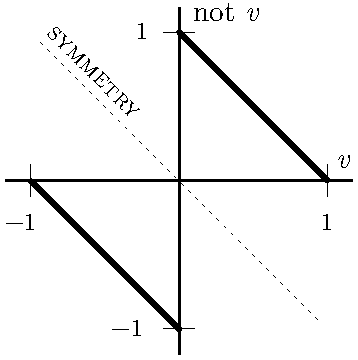
\includegraphics[width=\linewidth]{v_and_not_v.pdf}
\caption{The boundary and symmetry of reliability for a value $v$ and its negation \emph{not} $v$.}
\label{Figure:boundsym}
\end{marginfigure}
Since negative reliabilities are allowed, the formula becomes a little more complicated than just summing up reliabilities. 
For example, in a symmetrical and bounded body of information, if $\alpha = -0.75$ for $\bar{p}$ then $\beta = -0.25$ for $p$ using boundary, and using symmetry that is equivalent to $0.25$ for $\bar{p}$, which using boundary again yields the reliability of $p$ as $0.75$. The symmetry and boundary of values and their negation can be illustrated as a graph, seen in \figurename~\ref{Figure:boundsym}.

There is still no characteristic preventing a positor from having a multitude of reliabilities for the same posit at the same time. Such a quality will also ensure that even though the reliabilities $-0.25$ and $0.75$ for a posit produce equivalent assertions, only one should exist in the body of information\footnote{This avoids lunatic statements such as \enquote{I think Archie had a red beard and I am also sure he had a red beard, but he might not have had a red beard}.}.

\deffy{def. of exclusive}{%
A body of information is said to be \emph{exclusive} iff no assertions in which only the reliability differs exist.
}{exclusive}

An exclusive body of information prevents a positor from being, for example, certain of a fact and its opposite at the same time. Different positors may be in disagreement though, provided that it can be ensured that positors are having opinions about the same things. If one positor is saying that \enquote{Archie has a fluffy red beard} and another that \enquote{Archie was clean shaved}, can we be sure they are talking about the same Archie and how do we know \enquote{\emph{has beard}} means the same thing for them?

\deffy{def. of universal}{%
A body of information is said to be \emph{universal} iff positors agree on all appearances. 
}{universal}

In a universal body of information positors are not allowed to interpret, for example, the appearance $(A, \textit{has beard})$ differently\footnote{In order to disagree, there must still be a base upon which you agree, since how would you otherwise know what you are disagreeing about?}. Whatever the components represent will be the same for every positor. As assertions are predicates it is only through their representation that it can be determined if they are true or false. In order to have \enquote{meaningful} assertions, the bodies of information discussed henceforth will therefore be assumed to have all the previously defined characteristics.

\deffy{def. of comprehensive}{%
A body of information is said to be \emph{comprehensive} iff it is symmetric, canonical, bounded, exclusive and universal. 
}{comprehensive}

From here on it will be assumed that all bodies of information discussed are comprehensive. In a sense, a comprehensive body of information can be said to be a body of well behaving information.

%%%%%%%%%%%%%%%% CORRECTIONS %%%%%%%%%%%%%%%%%%%
\subsection{Corrections}
%
It would be presumptuous to assume that any statement made is always correct. We all make mistakes, and when opinions change in such a way that a previous statement is erroneous, corrections have to be made and made losslessly. To be able to do corrections a particular, but intuitively understandable, reliability value is needed. 

\deffy{def. of the complete uncertainty}{%
An assertion is called \emph{positive} when the reliability is above zero, \emph{negative} when below zero, and \emph{completely uncertain} when zero. 
}{uncertain}

Zero reliability is best understood through an example. Given the following posits: 
\begin{alignat*}{3}
p_{2} =[\{(A, \textit{has beard})\},\;&& \textrm{shaved clean},\;&& \textrm{10:02}] \\
\bar{p}_{2} =[\{(A, \textit{has beard})\},\;&& \textrm{not shaved clean},\;&& \textrm{10:02}] 
\end{alignat*}
For the posit $p_{2}$ and its opposite $\bar{p}_{2}$ the assertions $\assert(P, p_{2}, 0, T)$ and $\assert(P, \bar{p}_{2}, 0, T)$ are equivalent given symmetry. Since the reliability for the beard being both shaved clean and \emph{not} shaved clean is the same, the only meaningful interpretation is that zero reliability must be when the positor has no idea what the value is\footnote{It could be either of the posits, to any degree of certainty, but this positor does not know. Not knowing also conveys information, a fact that is often overlooked.}. The positor may have had an idea at some earlier time though.
\begin{alignat*}{3}
\assert(D, p_{2},\,&& 1,\,&& \textrm{Friday}) \\
\assert(D, p_{2},\,&& 0,\,&& \textrm{Sunday}) 
\end{alignat*}

In the assertions above Donna is changing her mind from on Friday thinking that Archie was shaved clean to on Sunday not having been able to tell whether Archie had a beard or not. The later assertion is called a retraction when it changes a positive or negative reliability for an earlier posit to zero.

\deffy{def. of a retraction}{%
Let $\mathbb{A}$ be a body of information. A \emph{retraction} is an assertion $\assert(P, p, 0, T') \in \mathbb{A}$ for which there exists an assertion $\assert(P, p, \alpha, T) \in \mathbb{A}$, with $\alpha \neq 0$ and $T < T'$.
}{retraction}

If at the same time another posit is asserted with non-zero reliability, this and the retraction together form a correction.

\deffy{def. of a correction}{%
Let $\mathbb{A}$ be a body of information. The three assertions $a_1 = \assert(P, p, \alpha, T)$, $a_2 = \assert(P, p, 0, T')$, and $a_3 = \assert(P, p', \alpha', T')$ together form a \emph{correction} when $\{a_1, a_2, a_3\} \subset \mathbb{A}$, $p \neq p'$, $\alpha \neq 0$, $\alpha' \neq 0$, and $T < T'$.
}{correction}

Extending the example with the assertion below, Donna says that it is possible that the perpetrator \enquote{Archie} had a fluffy red beard, while at the same time retracting her earlier assertion that his beard was shaved clean. 
\begin{align*}
p_{4} = [\{(A, \textit{has beard})\}, \textrm{fluffy red}, \textrm{10:02}] \\
\assert(D, p_{4}, 0.25, \textrm{Sunday}) 
\end{align*}

Without the retraction Donna would simultaneously be stating that Archie's beard is certainly shaved clean and also that it is possibly fluffy red, so she is contradicting herself. Both assertions will remain in effect without the retraction, but exactly why this is the case has yet to be formalized. 

%%%%%%%%%%%%%%%% INFORMATION IN EFFECT %%%%%%%%%%%%%%%%%%%
\subsection{The Information in Effect}
%
With both assertions and posits being bound in time, this warrants the question of what information actually is in effect at any given point in time. The intention is that posits should capture transitions of states in the domain being modeled, such as people finding themselves at the scene of a crime and later dispersed or Archie removing his fake beard, and assertions the transitions in the opinions expressed towards such posits. Assertion and appearance time give rise to two axes of time over which it should be possible to \enquote{travel}, where for all points in the bitemporal plane $\mathbb{T} \times \mathbbm{t}$ an unambiguous set of assertions should be in effect.

\deffy{def. of the information in effect}{%
Let $\mathbb{A}$ be a body of information. The \emph{information in effect} is a subset $\mathbb{A}(T_@, t_@) \subset \mathbb{A}$ given a bitemporal point in assertion and appearance time $(T_@, t_@) \in \mathbb{T} \times \mathbbm{t}$. Assuming $P$, $\alpha$, $T$, $D$, $v$, and $t$ are free variables, all assertions $\assert(P, p, \alpha, T) \in \mathbb{A}(T_@, t_@)$ with $p = [D, v, t]$ are found using the following selection criteria: 
\begin{criteria}
\item Let $\mathbb{A}_1 \subset \mathbb{A}$ be the assertions in $\mathbb{A}$ satisfying $T \leq T_@$ and $t \leq t_@$.
\item Let $\mathbb{A}_2 \subset \mathbb{A}_1$ be the assertions in $\mathbb{A}_1$ with $\alpha \neq 0$ and the latest appearance time $t$ for each combination of $P$ and $D$, excluding those assertions $\assert(P, p, \alpha, T)$ for which an assertion $\assert(P, p, 0, T_0)$ exists with $T \leq T_0 \leq T_@$.
\item Let $\mathbb{A}(T_@, t_@) \subset \mathbb{A}_2$ be the assertions from $\mathbb{A}_2$ with the latest assertion time $T$ for each combination of $P$, $D$, and $v$.
\end{criteria}
}{effect}

In less formal terms, the information in effect can be found by first rewinding all assertions to those whose assertion and appearance times are before the specified points in time. Among those, find the ones with the latest appearance times for each positor and dereferencing set, excluding retracted ones. Finally, keep those with the latest assertion times, again for each positor and dereferencing set. This will guarantee that a single assertion for each existing combination of a positor and a posit is in effect at any bitemporal point in time. In a sense, such a \enquote{slice} of assertions is static, since all temporal aspects have been removed by the operations described. Had it not been for the remaining reliability it would have been close to what is usually stored in a traditional database. Gathering some assertions from the running example:
\begin{alignat*}{3}
p_{1} = [\{(A, \textit{has beard})\},\;&& \textrm{fluffy red},\;&& \textrm{10:00}]  \\
p_{2} = [\{(A, \textit{has beard})\},\;&& \textrm{shaved clean},\;&& \textrm{10:02}]  \\
p_{3} = [\{(A, \textit{has beard})\},\;&& \textrm{shaved clean},\;&& \textrm{10:00}]  \\
a_1 = \assert(D, p_{2},\;&& 1,\;&& \textrm{Friday}) \\
a_2 = \assert(C, p_{1},\;&& 0.75,\;&& \textrm{Friday}) \\
a_3 = \assert(C, p_{3},\;&& -1,\;&& \textrm{Friday}) 
\end{alignat*}

Given the body of information above, $\{a_1, a_2, a_3\}$, the information in effect on $(\textrm{Saturday}, \textrm{10:01})$ is a set with two members $\{a_2, a_3\}$, as they are the only assertions with appearance times on or before 10:01 and assertion times on or before Saturday. The information in effect on $(\textrm{Saturday}, \textrm{10:03})$ is the set $\{a_1, a_2, a_3\}$, as all assertions are made before both times, and no retractions made. Although, something happened on Sunday, after Bella woke up:
\begin{alignat*}{3}
p_{4} = [\{(A, \textit{has beard})\},\;&& \textrm{fluffy red},\;&& \textrm{10:02}] \\
a_4 = \assert(D, p_{2},\;&& 0,\;&& \textrm{Sunday}) \\
a_5 = \assert(D, p_{4},\;&& 0.25,\;&& \textrm{Sunday}) 
\end{alignat*}

With this added information that extends the body of information, on $(\textrm{Sunday}, \textrm{10:03})$ the set $\{a_2, a_3, a_5\}$ is in effect. The assertion $a_1$ now has a corresponding retraction $a_4$ and must be excluded, which brings $a_5$ into effect. The two assertions, $a_2$ and $a_3$ made by Charlie are not contradictory, at the same time saying Archie's beard is probably fluffy red and certainly not shaved clean. In fact, \enquote{certainly not} may be stated for an arbitrary number of values without a positor contradicting itself\footnote{Note that there is a difference between stating that \enquote{Archie's beard is certainly not red} and \enquote{I have no idea if Archie's beard is red}. The former excludes a particular value and remains in the information in effect, whereas the latter leaves all doors open and is removed from the information in effect. Both may be stated for an arbitrary number of values without contradicting yourself though.}. But, what if the following assertion is made:
\begin{align*}
a_6 = \assert(D, p_2, -0.75, \textrm{Sunday}) 
\end{align*}

Suddenly, Donna is stating that Archie's beard is both possibly fluffy red and probably not shaved clean. Could it be the case that Donna is now contradicting herself? When the same positor is having several assertions in effect with the same dereferencing set, but different values and reliabilities, another characteristic is needed ensuring positors are non-contradictory.

\deffy{def. of non-contradictory}{%
A body of information is said to be \emph{non-contradictory} iff for every information in effect the reliabilities in all positive and negative assertions made by the same positor for the same dereferencing set satisfy the inequality: $$\frac{1}{2}\sum_{i = 1}^{n}\left[1 - \frac{\alpha_i}{|\alpha_i|}\right ] + \sum_{i = 1}^{n}\alpha_i \leq 1$$
}{contradictions}

Looking at $\{a_5, a_6\}$, these two assertions by Donna concurrently assert different values for the beard of Archie and they are both in effect on $(\textrm{Sunday}, \textrm{10:03})$. Calculating the left side of the inequality gives:
\begin{small}
$$\frac{1}{2}\left[1-\frac{0.25}{|0.25|}+1-\frac{-0.75}{|-0.75|}\right] + 0.25 - 0.75 = 0.5$$
\end{small}

From this is can be concluded that Donna is far from contradicting herself, since the reliabilities only \enquote{sum up} to 0.5. As another example, a positor may be 95 percent sure that Archie's beard is not shaved clean, and the same for up to 20 different beard styles and colors, without being contradictory. The \nth{21} beard style Archie has almost certainly not got, however, will bring the left hand side to 1.05. Taking this example all the way, a positor may simultaneously assert with 100 percent certainty that something is \emph{not} the case for an unlimited number of posits.

\deffy{def. of indecisive and decisive}{%
When multiple assertions by the same positor are in effect for different posits with the same dereferencing set, the positor is said to be \emph{indecisive} with respect to the set. When a single assertion of a positor is in effect for a dereferencing set, the positor is said to be \emph{decisive} with respect to the set. The information in effect is said to be \emph{indecisive} if there is at least one indecisive positor and \emph{decisive} if not. A body of information is said to be \emph{decisive} if for every information in effect no indecisive positors exist and \emph{indecisive} if there is at least one indecisive positor.
}{decisiveness}

Since contradictions by definition rely on indecisiveness, it follows that a body of information which is decisive is always non-contradictory.\footnote{A traditional relational database is decisive as no possible alternative values can be represented, without modeling such behavior explicitly.}

%%%%%%%%%%%%%% REASSERTIONS AND RESTATEMENTS %%%%%%%%%%%%%%%%%%%%%
\subsection{Reassertions and Restatements}
%
In a traditional database, updating a value to the same value is an indistinguishable operation, since the value will remain the same after the operation is completed. For assertions, it is possible to assert the exact same thing over and over again with increasing assertion times. Such assertions can be chosen to be kept or discarded, depending on the requirements at hand. 

\deffy{def. of a reassertion and assertive}{%
If two in assertion time successive assertions are otherwise equal, the later is said to be a \emph{reassertion} of the earlier. A body of information is said to be \emph{assertive} if reassertions exist.
}{assertive}

It may be noted that in an assertive body of information, the information in effect will contain the latest reassertion, and if desired further searching is necessary in order to find the first assertion in a chain of reassertions. To further exemplify, Charlie will make three additional assertions, $\{a_7, a_8, a_9\}$:
\begin{alignat*}{3}
p_{1} = [\{(A, \textit{has beard})\},\;&& \textrm{fluffy red},\;&& \textrm{10:00}]  \\
p_{4} = [\{(A, \textit{has beard})\},\;&& \textrm{fluffy red},\;&& \textrm{10:02}] \\
a_2 = \assert(C, p_{1},\;&& 0.75,\;&& \textrm{Friday}) \\
a_7 = \assert(C, p_{4},\;&& 0.75,\;&& \textrm{Friday}) \\
a_8 = \assert(C, p_{1},\;&& 0.75,\;&& \textrm{Sunday}) \\
a_9 = \assert(C, p_{4},\;&& 0.25,\;&& \textrm{Sunday}) 
\end{alignat*}
 
Here the assertion $a_8$ is a reassertion of $a_2$, since only the assertion time differs. The assertions $a_7$ and $a_2$ share a different relationship though, where the assertion time is the same, but the appearance time differs while the dereferencing set and value is the same in the posit.
 
\deffy{def. of a restatement and restatable}{%
For two assertions, $\assert(P, p, \alpha, T)$ and $\assert(P, p', \alpha, T)$, with $p = [D,v,t]$ and $p' = [D,v,t']$, such that $t < t'$, the latter is called a \emph{restatement} of the former. If a body of information contains restatements it is said to be \emph{restatable}.
}{restatable}

Given the definition above, the assertion $a_7$ is a restatement of $a_2$, but $a_9$ is not a restatement of $a_8$ as the reliability differs. Looking at $a_9$ and $a_7$, Charlie is also downgrading his belief in the posit, from being probable that the beard was fluffy red to only possible that is was. Perhaps he observed Archie for the full two minutes between 10:00 and 10:02, but could not at first believe his eyes that the beard was gone. With some afterthought, he was less sure on Sunday. The beard was probably fluffy red at 10:00 and only possibly fluffy red at 10:02, according to Charlie. 


 %%%%%%%%%%%%%%%% MODELING %%%%%%%%%%%%%%%%%%%
\section{Modeling and Typing}
%
While the posits and assertions seen so far have been intuitively understandable, being constructed from a story and simple examples, the exact nature of Archie is still undecided. Is it a perpetrator, an accused, a person, a human being, a fictional character, or something completely different? In order to determine what unique identifiers actually represent, a model is needed. Models provide auxiliary information, with the aim to collate similar things under common names. The more well understood such names are the more intelligible the model becomes\footnote{However, even if positors agree upon such names, they may disagree on how to assign them, or in other words, the same information may have many models.}.

\deffy{def. of a classifier and a class}{%
Let $\textit{is class}$ be a role reserved for the purpose of modeling. A posit $p_c = [\{(\mathcal{C}, \textit{is class})\}, c, t]$, defines the name of a \emph{class} through the string $c$ and associates the unique identifier $\mathcal{C}$ with it. A \emph{classifier} is a relationship that binds a thing to a class, expressed through posits on the form $p_{\mathbb{M}} = [\{(i, \textit{thing}), (\mathcal{C}, \textit{class})\}, v, t]$.
}{classifier}

The defined strings are intended to represent classifications, such that it can be determined to which class any unique identifier belongs. Thanks to the time point $t$ in the classifier, the class of $i$ may change, naturally, over time. First given some posits that define class names assumed to have existed since the beginning of time, here denoted by $-\infty$, the following posits may all be valid classifiers for Arthur: 
\begin{alignat*}{3}
p_{c1} = [\{(\mathcal{C}_1, \textit{is class})\},\;&& \textrm{Infant},\;&& -\infty] \\
p_{c2} = [\{(\mathcal{C}_2, \textit{is class})\},\;&& \textrm{Teenager},\;&& -\infty] \\
p_{\mathbb{M}1} = [\{(A, \textit{thing}), (\mathcal{C}_1, \textit{class})\},\;&& \textrm{active},\;&& \textrm{1972}] \\
p_{\mathbb{M}2} = [\{(A, \textit{thing}), (\mathcal{C}_1, \textit{class})\},\;&& \textrm{inactive},\;&& \textrm{1973}] \\
p_{\mathbb{M}3} = [\{(A, \textit{thing}), (\mathcal{C}_2, \textit{class})\},\;&& \textrm{active},\;&& \textrm{1985}] 
\end{alignat*}

From these it is apparent that two classifications exist and have always existed\footnote{Posits that define class names from the beginning of time may in some sense be viewed as being \emph{static}, or in other words, have no way to naturally change into a different value.}, and that Arthur was an infant between 1972 and 1973 and became a teenager in 1985. However, it would be equally valid to at all those times state that Arthur is a person, as illustrated by the following posits. 
\begin{alignat*}{3}
p_{c3} = [\{(\mathcal{C}_3, \textit{is class})\},\;&& \textrm{Person},\;&& -\infty] \\
p_{\mathbb{M}4} = [\{(A, \textit{thing}), (\mathcal{C}_3, \textit{class})\},\;&& \textrm{active},\;&& \textrm{1972}] 
\end{alignat*}

This hints at a relationship between infant and person, since Arthur is both an infant and a person during the year of 1972, which of course can be expressed through its own posit.
\begin{alignat*}{3}
p_{\mathbb{M}4} = [\{(\mathcal{C}_1, \textit{subclass}), (\mathcal{C}_3, \textit{class})\},\;&& \textrm{active},\;&& -\infty] 
\end{alignat*}

Whatever needs to be said about classes and how they relate to each other and other things can be expressed using posits. These can be indefinitely extended by introducing new reserved strings used in their appearances. Each class could have description, for example, through the $(\mathcal{C}, \textit{has description})$ appearance. Just like posits in general, classifiers are meaningless unless asserted by a positor, acting as a modeler in this case. A modeler may, like positors in general, disagree on the model, or express uncertainty towards parts of it. 
\begin{alignat*}{4}
a_{\mathbb{M}1} = \assert(&&M, p_{\mathbb{M}1},\;&& 0.75,\;&& \textrm{Today}) \\
a_{\mathbb{M}1} = \assert(&&M, p_{\mathbb{M}4},\;&& 1,\;&& \textrm{Today}) \\
a_{\mathbb{M}1} = \assert(&&L\;, p_{\mathbb{M}4},\;&& -1,\;&& \textrm{Today}) 
\end{alignat*}

The modeler $M$ is quite sure that Arthur was an infant since 1972, while simultaneously sure that Arthur is a person, whereas $L$ is certain Arthur is not a person. This does not necessarily mean that Arthur is an alien, unless $L$ models it so, but that $L$ may have chosen a model in which Arthur perhaps is a client instead\footnote{From the point of view of a lawyer in the case, this is not unreasonable.}. 

\deffy{def. of a model}{%
Let $\mathbb{A}$ be a body of information and let $\mathbb{I}$ be the set of all unique identifiers found in $\mathbb{A}$. The \emph{model} $\mathbb{M}$ of $\mathbb{A}$, denoted $\mathbb{M} \models \mathbb{A}$, is a comprehensive body of information in which each positor exhaust $\mathbb{I}$ through assertions of classifiers.
}{model}

A model, then, contains complete information about which class every thing belongs to. It may contain much more information, such as detailed descriptions of classes or how classes relate to each other, through for example inheritance. It contains information about information and can be seen as meta-information with respect to the body of information it models. If the two are intermixed it is important to keep track of which strings have been reserved for use in those appearances that pertain to modeling.

As can be understood from the examples, there may be many ways to model the same body of information. The question then arises when a model is a \enquote{good} model. Unfortunately there is no simple answer. In some cases, few and generic classes are preferable, where in others many and specific ones are better. A model is that which creates boundaries between similar and dissimilar things. To model is to define these boundaries by determining when things are similar enough to be of the same class. Assuming that Arthur belongs to the person class and that many other things also are persons, it is possible to derive some additional information about persons from the posits in which such things appear. Backtracking from $p_{c3}$ it is possible to find all posits in which things of the person type appears, many of which will have similar structures.

\deffy{def. of a posit type}{%
A \emph{posit type}, $\typeof{p} = [\{(\mathcal{C}_1, r_1), \ldots, (\mathcal{C}_n, r_n)\}, \typeof{v}, \typeof{t}]$, for a posit $p = [\{(i_1, r_1), \ldots, (i_n, r_n)\}, v, t]$, is a structure constructed by replacing unique identifiers, $i_i$ with the unique identifiers of their class, $\mathcal{C}_i$, the value, $v$, with its data type, $\typeof{v}$, and the time point, $t$, with its data type, $\typeof{t}$.
}{posittype}

Posit types are descriptive by nature, and will be used to further enrich the model. For example, given the person class, an example posit and its corresponding type are:
\begin{align*}
p_{4} =\;& [\{(A, \textit{has beard})\}, \textrm{fluffy red}, \textrm{10:02}] \\
\typeof{p_{4}} =\;& [\{(\mathcal{C}_3, \textit{has beard})\}, \mathsf{string}, \mathsf{time}] 
\end{align*}

We know from $p_{c3}$ that $\mathcal{C}_3$ is the person class. It appears then that persons may have beards of some string value capturing its color and since some specified time.

\deffy{def. of a typing and a type}{%
Let $\textit{is type}$ be a role reserved for the purpose of creating types. A posit $p_{\tau} = [\{(\mathcal{T}, \textit{is type})\}, \tau(p), t]$, defines a \emph{type} through the posit type $\tau(p)$ and associates the unique identifier $\mathcal{T}$ with it. A \emph{typing} is a relationship that binds a class to a type, expressed through posits on the form $p_{\mathbb{T}} = [\{(\mathcal{C}, \textit{class}), (\mathcal{T}, \textit{type})\}, v, t]$.
}{typing}

Defining a type is done by binding a unique identifier to a posit type, for example $\typeof{p_{4}}$, using another posit\footnote{Remember that posits are defined to bind unique identifiers to values that may be of any data type, primitive as well as complex ones. A posit type can be considered to be a complex data type in this case.}. 
\begin{align*}
p_{\tau4} =\;& [\{(\mathcal{T}_1, \textit{is type})\}, \typeof{p_{4}}, -\infty] \\
p_{\mathbb{T}1} =\;& [\{(\mathcal{C}_3, \textit{class}), (\mathcal{T}_1, \textit{type})\}, \textrm{commonly}, \textrm{1942}]
\end{align*}

Using the value in a typing, it is possible to express more than just if the relationship is currently active or inactive. It can be used to indicate how often a person has a beard in general, and which in the example above is \emph{commonly}. Other thinkable values that can be useful are \emph{rarely}, \emph{always}, and \emph{never}\footnote{When values form an enumeration, it is important that they together are mutually exclusive and exhaustive, which is why \emph{never} is needed, since it thinkable that it will become impossible for persons to have beards from some point in time.}. These may change over appearance time if the demographics of the persons in the universe of discourse changes.  It is important to note that even if one bearded person exists it does not imply that all persons can or must have beards. There will be no posits of type $\typeof{p_{4}}$ for Bella or Donna, ever. 

Typings are created from the information at hand and they evolve along with the information, and should therefore not be seen as templates into which future information should fit. Types and typings are asserted by positors, just like classes and classifiers, even if types are somewhat harder to disagree upon, but it is possible for two different positors to have a difference in opinion about the data types involved. Extending the example we know Archie and Bella was observed by Charlie at the scene of the crime, but there seems to have been something preceding the crime, involving Xavier.
\begin{align*}
p_{5} =\;& [\{(A, \textit{is accused}), (B, \textit{is victim}), (C, \textit{is witness})\}, \\
&\textrm{at scene of crime}, \textrm{09:58}] \\
p_{6} =\;& [\{(A, \textit{is accused}), (X, \textit{is victim}), (C, \textit{is witness})\}, \\
&\textrm{at scene of crime}, \textrm{09:42}] 
\end{align*}

Given the similarities in the structure of the posits $p_{5}$ and $p_{6}$, it would be reasonable to assume they have the same posit type, but that is actually not the case. What seems to have started the kerfuffle between Archie and Bella was in fact that Archie was being mean to her dog, Xavier, which Charlie witnessed somewhat earlier that day. This results in two similar, but not equal, posit types $\typeof{p_{5}}$ and $\typeof{p_{6}}$.
\begin{align*}
p_{c4} =\;& [\{(\mathcal{C}_4, \textit{is class})\}, \textrm{Animal}, -\infty] \\
p_{\mathbb{M}5} =\;& [\{(X, \textit{thing}), (\mathcal{C}_4, \textit{class})\}, \textrm{active}, \textrm{2009}] \\
\typeof{p_{5}} =\;& [\{(\mathcal{C}_3, \textit{is accused}), (\mathcal{C}_3, \textit{is victim}), (\mathcal{C}_3, \textit{is witness})\}, \\
&\mathsf{string}, \mathsf{time}] \\
\typeof{p_{6}} =\;& [\{(\mathcal{C}_3, \textit{is accused}), (\mathcal{C}_4, \textit{is victim}), (\mathcal{C}_3, \textit{is witness})\}, \\
&\mathsf{string}, \mathsf{time}] \\
p_{\tau5}' =\;& [\{(\mathcal{T}_2, \textit{is type})\}, \typeof{p_{5}}, -\infty] \\
p_{\tau6}' =\;& [\{(\mathcal{T}_3, \textit{is type})\}, \typeof{p_{6}}, -\infty] \\
p_{\mathbb{T}2} =\;& [\{(\mathcal{C}_3, \textit{class}), (\mathcal{T}_2, \textit{type})\}, \textrm{rarely}, \textrm{1942}] \\
p_{\mathbb{T}3} =\;& [\{(\mathcal{C}_3, \textit{class}), (\mathcal{T}_3, \textit{type})\}, \textrm{rarely}, \textrm{1942}] 
\end{align*}

This example illustrates the importance of typing. The added information it gives makes it possible to get the whole picture of what is going on, and while the posits $p_5$ and $p_6$ may look alike, the things they relate differ in their classes. To get a good understanding of what a class represents it is useful to look at a particular set, called an ensemble.

\deffy{def. of an ensemble}{%
Let $\mathbb{A}$ be a body of information. If $\mathcal{C}$ is the unique identifier for a class $c$ from a model of $\mathbb{A}$, the \emph{ensemble} of $c$ is the information in effect limited to all assertions of typings in which $\mathcal{C}$ occurs. 
}{ensemble}

An ensemble gives a good idea of what it entails to be an instance of, for example, the \enquote{Person} class. You may even say that a person is that which commonly may have a beard, always has a gender and a birth date, and that rarely is involved as an accused, victim, or witness, where the victim could be an animal or another person\footnote{Provided that some positor has asserted these typings.}.

While sufficient to provide a model through a set of classifiers, the ensembles enrich the model by providing a more descriptive view of each class. Ensembles will naturally evolve over time, as new information is added. Together they can be likened with a growing schema in a database, but with a complete history of changes, and possibly multiple conflicting models and typings of the same information.

 %%%%%%%%%%%%%%%% IDENTIFICATION %%%%%%%%%%%%%%%%%%%
\subsection{Identification}
%
A body of information is rarely something that comes about in a Big Bang kind of fashion. Rather, they are gradually built, and many may continue to evolve indefinitely. Herein lies a difficulty with the unique identifiers that have already been assigned within that body. Say, if a new witness steps forward a few weeks later, is the Archie that witness saw the same Archie that already has been assigned the unique identifier $A$? 

\deffy{def. of an identification}{%
Let $c$ be a class in a body of information $\mathbb{A}$ and $e$ its ensemble. Given some circumstances, where circumstances consist of information not yet or only partly represented in $\mathbb{A}$, an \emph{identification} is a search in $A$ in which $e$ is gradually populated with values and/or other unique identifiers, until they match existing assertions and posits, from some information in effect, such that a single unique identifier of class $c$ can be determined or that after exhausting the circumstances no match was found.
}{identification}

In the case of the new witness, the circumstances may have been that that witness also saw a man at the same scene of the crime at the same time as the others and that that man also wore a red beard and fled shortly thereafter. This may have been deemed sufficient to draw the conclusion that the new witness must be talking about the same man, Archie. When ensembles are large, have many members in their sets, it may be convenient to narrow down searches by providing some subsets of posit types that normally suffice for identification.

\deffy{def. of an identifier}{%
Let $e$ be the ensemble of a class $c$. An \emph{identifier} of $c$ is a subset $e_{id} \subset e$, for which it is deemed sufficient to fill with values and/or other unique identifiers in order to complete an identification.
}{identifier}

Identification is, by all means and the definitions above, no exact science. There also may be many ways to reach the same conclusion in an identification and many different identifiers for the same class. A real perpetrator could perhaps be identified through DNA matching, fingerprints, witnesses, motives, means, opportunity, and so on. Since positors are allowed to make retractions, this may make identification even harder. 

\deffy{def. of analytic and synthetic}{%
Let $p$ be a posit in which the unique identifier $i$ appears. If all positors retract $p$ and this is debilitating to the identification process, then $p$ is said to be \emph{analytic} to $i$ and \emph{synthetic} otherwise.
}{anasyn}

To illustrate these concepts, assume that Eliot, the investigator, swabbed Archie shortly after capturing him, resulting in his DNA being sequenced. 
\begin{alignat*}{3}
p_{7} = [\{(A, \textit{has DNA})\},\;&& \texttt{ACGT\ldots},\;&& \textrm{1972-08-20}]  \\
a_{10} = \assert(E, p_{7},\;&& 1,\;&& \textrm{Sunday}) 
\end{alignat*}

If Eliot retracts $a_{10}$ and this would seriously debilitate the identification process, that means that Archie's DNA is analytic to Archie. Analytic posits need to be handled with additional care as the information evolves, since retracting them may have negative side effects\footnote{In some modeling techniques, identifiers consisting of only analytic posits are called \enquote{candidate keys}.}. Assuming that it was the DNA of Archie that eventually led to his conviction, the whole trial may be put in question if it turns out that the DNA actually belonged to someone else.

 %%%%%%%%%%%%%%%% CARDINALITY %%%%%%%%%%%%%%%%%%%
\subsection{Cardinality}
%

Eliot's investigation would also show that Archie and Bella knew each other quite well. The posits below\footnote{These posits describe a quaternary relationship. While high arity relationships are not often seen in database models, they actually appear quite frequently in real life. The discrepancy could perhaps be explained by the simple fact that they are harder to manage, but then, what is lost in databases due to this fact is quite troublesome.} describe a series of events, from Bella marrying Archie in 2004, to divorcing him in 2009, and to both remarrying others in 2012. Of these, only the first two constitute a real change, since they have the same dereferencing set. The last two instead constitute different events, as the dereferencing sets involve different unique identifiers. 
\begin{alignat*}{3}
p_{1w} =\;& [\{&(&A, \textit{is husband}),(B, \textit{is wife}),(C, \textit{is minister}), \\
&&(&8, \textit{is church})\}, \textrm{marriage}, 2004] \\
p_{2w} =\;& [\{&(&A, \textit{is husband}),(B, \textit{is wife}),(C, \textit{is minister}), \\
&&(&8, \textit{is church})\}, \textrm{divorce}, 2009] \\
p_{3w} =\;& [\{&(&A, \textit{is husband}),(F, \textit{is wife}),(C, \textit{is minister}), \\
&&(&8, \textit{is church})\}, \textrm{marriage}, 2012] \\
p_{4w} =\;& [\{&(&G, \textit{is husband}),(B, \textit{is wife}),(C, \textit{is minister}), \\
&&(&9, \textit{is church})\}, \textrm{marriage}, 2012] 
\end{alignat*}

With combined temporality, concurrency, and reliability, it is of interest to understand constraints under the circumstances where values may change over time, positors may be in conflict, and retractions occur. Describing the specific case of cardinality in transitional modeling, which is a common constraint in almost every technique, will help shed light on the general case of how any constraint is handled. Consider enforcing monogamy\footnote{The author is well aware that weddings and marriages can take many other forms and is in this example expressing no particular preference, but for the sake of simplicity the examples look the way they do.} in the \enquote{wedding} relationship, where a married couple may come to divorce, different positors may have conflicting opinions about when it happened, and they may change their minds about whether it happened at all.   

\deffy{def. of a limiter}{%
A \emph{limiter} is a triple, $(R, l, u)$, where $R = \{r_1, \ldots, r_n\}$ is a set of strings and $l$ and $u$ are positive integers, with the special value $*$ also allowed for $u$. If $u = *$, then $l$ may be any positive integer, or otherwise $l \le u$ must hold.
}{limiter}

The intention of a limiter is to express a lower, $l$, and upper, $u$, bound for how many times a unique identifier or combination thereof may appear having the roles from $R$ in a relationship. The special value $*$ should be interpreted as an \enquote{unlimited} number of times\footnote{Note that zero is not a valid value for the lower bound. Because of the way posits are defined, they always contain unique identifiers with every role in a dereferencing set. In that respect, if the church is optional at a wedding, a different posit type without the \textit{is church} role would be used.}.

\deffy{def. of a cardinality constraint}{%
A \emph{cardinality constraint}, $\{L_1, \ldots, L_n\}$ with $n > 1$ over a posit type, $\typeof{p}$, that has more than one role, is a set of limiters, $L_i = (R_i, l_i, u_i)$, with $R_i = \{r_{i_1}, \ldots, r_{i_m}\}$ for which every $r_{i_j}$ is a role in the posit type $\typeof{p}$ and where $R_i$ are disjoint sets.
}{constraint}

In order to enforce monogamy, first recognize that all posits share the same posit type $\typeof{p_{w}}$. Assuming that $\mathcal{C}_5$ is the unique identifier for the \enquote{Location} class, the posit type for the wedding relationship becomes as follows.
\begin{alignat*}{3}
\typeof{p_{w}} =\;& [\{&(&\mathcal{C}_3, \textit{is husband}), (\mathcal{C}_3, \textit{is wife}), (\mathcal{C}_3, \textit{is minister}), \\ 
&&(&\mathcal{C}_5, \textit{is church})\}, \mathsf{string}, \mathsf{year}]
\end{alignat*}

Preventing a husband from having several wives and wives from having several husbands needs the following cardinality constraint on $\typeof{p_{w}}$. 
\begin{align*}
\{(\{\textit{is husband}\}, 1, 1), (\{\textit{is wife}\}, 1, 1)\}
\end{align*}

According to the limiters, the unique identifier for a husband must appear at least once and at most once at the same time as the unique identifier for a wife also must appear exactly once. This enforces a one-to-one relationship between husbands and wives. However, already the first two posits, $p_{1w}$ and $p_{2w}$, seem to break this constraint, since both Arthur and Bella appear in both of them. 

\deffy{def. of decisive fulfillment}{%
A cardinality constraint is said to be \emph{fulfilled} in a decisive body of information, if among posits that share the same type $\typeof{p_1} = \typeof{p_2} = \ldots = \typeof{p_n}$, unique identifiers appear at least $l$ times and at most $u$ times in the roles specified in the corresponding limiter, for each positor and every information in effect.
}{deful}

This is where it is important to notice that constraint checks are not made against all posits in a body of information, but rather made for each positor and information in effect in that body. Fulfillment, as can be seen, is only defined for decisive bodies of information. Fulfillment in indecisive bodies will not be detailed in this paper, but to give an idea, if Eliot asserts with 0.50 reliability both that Archie is currently married either to Bella or to Fanny, he could be stating that there is a chance Archie is married to both of them or that in reality, one wife is a fact and the other is not, but he is not sure which one it is. Cardinalities in indecisive bodies of information may aid in resolving this ambiguity, but therefore also need additional treatment, which is left as further research. Now, let Eliot instead decisively assert the posits. 
\begin{align*}
a_{1w} = \assert(E, p_{1w}, 1, \textrm{Sunday}) \\
a_{2w} = \assert(E, p_{2w}, 1, \textrm{Sunday}) \\
a_{3w} = \assert(E, p_{3w}, 1, \textrm{Sunday}) \\
a_{4w} = \assert(E, p_{4w}, 1, \textrm{Sunday}) 
\end{align*}

The information in effect on $(\textrm{Sunday}, 2004)$ is $\{a_{1w}\}$, on $(\textrm{Sunday}, 2009)$ it is $\{a_{2w}\}$, and on $(\textrm{Sunday}, 2012)$ it is $\{a_{3w}, a_{4w}\}$, exhausting the entire bitemporal timeline. Neither of these break the constraint, so the constraint is therefore fulfilled. Let Both Archie and Bella admit they were married in 2004 through the following two assertions.
\begin{align*}
a_{5w} = \assert(A, p_{1w}, 1, \textrm{Sunday}) \\
a_{6w} = \assert(B, p_{1w}, 1, \textrm{Sunday}) 
\end{align*}

Each of the sets with the information in effect above will now also have these two assertions included. This will, however, still not break the constraint, since each assertion that could have done so is made by a different positor. This pattern repeats itself for any type of constraint, such that checks are made for each positor and information in effect\sidenote[][-5cm]{A uniqueness constraint, such that the client number at a law firm may never repeat itself and thereby uniquely identify a client, is also only checked against the information in effect and for each positor. Two different positors may assign the same client number to two different clients and the same client number may have been reused for another client at a different time in the past.}. 

Given the quaternary \enquote{wedding} relationship, there are a lot more cardinality constraints that can be defined. For the sake of completeness, the following is defined. 

\deffy{def. of complete cardinality\footnote{The size of the complete set is calculated by: 
\begin{align*}
\frac{3^n-2^{n+1}+1}{2}\qquad
\end{align*} giving for example 3, 6, 25, 90, and 301 elements for 2, 3, 4, 5, and 6-ary posits. The fraction is the same as the number of matches $n$ players would play, given that all possible teams, combining them in sizes from $1$ to $n-1$, meet once and that players cannot meet themselves.}}{%
The \emph{complete cardinality} of a posit type, $\typeof{p}$, is a set of all cardinality constraints that can be created using combinations of roles from $\typeof{p}$.
}{cardinality}

Already for a quaternary relationship like the wedding, the complete cardinality set has 25 members. Along with three already exemplified, another five of them are the following constraints.
\begin{align*}
\{(\{\textit{is husband}\}, 1, *),\;& (\{\textit{is minister}\}, 1, 1)\}, \\
\{(\{\textit{is wife}\}, 1, *),\;& (\{\textit{is minister}\}, 1, 1)\}, \\
\{(\{\textit{is husband}\}, 1, *),\;& (\{\textit{is church}\}, 1, 1)\}, \\
\{(\{\textit{is wife}\}, 1, *),\;& (\{\textit{is church}\}, 1, 1)\}, \\
\{(\{\textit{is husband, is wife}\}, 1, *),\;& (\{\textit{is minister, is church}\}, 1, 1)\}
\end{align*}

The first two constraint expresses that if a husband or wife is present at a wedding exactly one minister must be as well and that a minister may wed many husbands and wives. The second two expresses a similar constraint with respect to the church. The last expresses that if a husband and a wife is present at a wedding in which there is a combination of a minister and a church, there must be only one such combination, and that a combination of a minister and a church may have partaken in the wedding of many husbands and wives. 

Intuitively, there should be some relation between the first four constraints and the last. It is counter-intuitive that a husband and wife could be married more than once if only they find a new combination of minister and church. While not immediately obvious how, it turns out that it is possible to calculate the smallest and largest possible bounds for the last constraint, given the first four. Being slightly less formal in how this is calculated, first, define a \enquote{cross product} according to the following rules for the lower and upper bounds in a cardinality constraint.
\begin{align*}
(l_i, u_i)\times (l_j, u_j) &= (max(l_i, l_j), min(u_i, u_j)) 
\end{align*}

Since the upper bound can have the special $*$ value, $max$ and $min$ are defined as follows when it is involved.
\begin{align*}
min(u, *) &= u \\
max(l, *) &= l \\
min(*, *) &= max(*, *) = * 
\end{align*}

To find the bounds for the last constraint, first calculate from left to right and crosswise roles, (husband side to minister) $\times$ (husband side to church) $\times$ (wife side to minister) $\times$ (wife side to church) = $(1,~*) \times (1,~*) \times (1,~*) \times (1,~*) = (1,~*)$. Then calculate from right to left and crosswise roles, (minister side to husband) $\times$ (minister side to wife) $\times$ (church side to husband) $\times$ (church side to wife) = $(1,~1) \times (1,~1) \times (1,~1) \times (1,~1) = (1,~1)$. This gives the bounds found in the last constraint, and it cannot pass beyond these bounds without resulting in inconsistent cardinalities. Further restricting the constraint is allowed though, and warrants the need for actually specifying higher order constraints. For example, if a minister is only allowed to wed five couples in any given church before finding a new church, the last constraint can be restricted to:
\begin{align*}
\{(\{\textit{is husband, is wife}\}, 1, 5),\;& (\{\textit{is minister, is church}\}, 1, 1)\}
\end{align*}

\pagebreak\deffy{def. of a limiting and a limit}{%
Let $\textit{is limit}$ be a role reserved for the purpose of creating constraints. A posit $p_{L} = [\{(\mathcal{L}, \textit{is limit})\}, L, t]$, defines a \emph{limit} through the limiter $L$ and associates the unique identifier $\mathcal{L}$ with it. A \emph{limiting} is a relationship that binds a posit type to a limit, expressed through posits on the form $p_{\mathbb{L}} = [\{(\mathcal{T}, \textit{type}), (\mathcal{L}, \textit{limit})\}, v, t]$.
}{limiting}

When limitings are asserted, constraints also become part of the information itself, similar to the model and the types. This makes it possible for constraints to be valid only during certain periods of time, for example, or that they may evolve and look different now from what they did before. Different positors may also simultaneously use different constraints. 

Declaring constraints in transitional modeling turns out to be very similar to traditional techniques, where the complexity instead lies within their enforcement, over every positor and every information in effect. 


%%%%%%%%%%%%%%%% RELATED RESEARCH %%%%%%%%%%%%%%%%%%%
\section{Related Research}
%
Some 20 years ago~\parencite{Inmon} defined a Data Warehouse as being \enquote{a subject-oriented, integrated, time-variant, nonvolatile collection of data}. While companies are belatedly coming to terms with the first two conditions, in our experience, supported by~\parencite{GolfarelliRizzi}, few can say that they fulfil the last two, primarily because of lacking methods. If Data Warehouses are our best attempt at integrating bodies of information under evolution, they are currently not well equipped to do so. To address this the presented \emph{transitional modeling} technique, rooted in multiple research areas, makes it easy to communicate, store, manage, and analyze information that is conflicting, uncertain and varying.

\parencite{Bradley} shares the notion that a thing is defined by its appearance and change is \enquote{a bond of identity in differences}. Through positors and appearances problems such as \enquote{the Ship of Theseus}, discussed by~\parencite{Chisholm}, can be largely avoided. Even if every plank in the ship is replaced, the unique identifier once associated with the ship will prevail, and will do so eternally~\parencite{Sider, Black}. If at some point another identifier is associated with the ship, because a different positor deems it a new ship, that positor is perfectly free to do so. The two ships can then be discussed in parallel, and relations between them defined. To paraphrase the greek philosopher Heraclitus [\textasciitilde500 BC], it is possible for the same man to step into the same river twice, as long as some positor can identify them to still be the same. Being the same man or the same river rarely comes down to following the trail of body cells or water molecules.

\parencite{Lombard} presents the problem of distinguishing relational from non-relational change, which is solved by separating immutable parts, allowing change to happen independently across a model, similar to how our unique identifiers are the only immutables, while everything else may change. \parencite{MoensSteedman} define \enquote{culmination} as being a point in time \enquote{accompanied by a transition to a new state of the world}, similar to how our appearance time is used to capture different states. \parencite{Bradley} also states that shifting to statements and away from reality relaxes the need for absolute truth. Similarly our assertions make it possible to hold different and uncertain opinions about posits. An RDF triple~\parencite[-4mm]{RDF} roughly corresponds to our posit, but has no concept beyond it with respect to temporality, reliability, or concurrency. The quality of a posit being \enquote{analytic} or \enquote{synthetic} is borrowed directly from the philosophical works of~\parencite{Ayer, Ramsey}. 

\parencite{Johnston} suggests an approach based on speech act theory with actors resembling positors and speech acts bound to two axes of time, but does not take reliability into account. \parencite{Reichenbach} was among the first to suggest bitemporality; a difference between the \enquote{point of speech} and the \enquote{point of event}, similar to our assertion time and appearance time. The specifics of bitemporal models in databases was later elaborated upon by~\parencite{Snodgrass}. Neither Reichenbach nor Snodgrass touch upon conflicting or uncertain information.

Reliability has likenesses with the Uncertainty Theory of~\parencite{Liu} and its personal belief degree. While Liu states that \enquote{when the personal knowledge changes, the belief degree changes too}, and that \enquote{different people may produce different belief degrees}, his theory does not as of yet support these notions. His \enquote{normality} and \enquote{duality} axioms correspond to our definitions of non-contradiction and boundary, although with a symmetry around $0.5$ instead of $0$ as used in transitional modeling.

\parencite{MassaroEtAl, LinEtAl} highlight the difficulty of integrating information from multiple sources, especially when these may be contradictory. The problem of integration lies in the fact that it is treated at write time, such that integrated information end up being stored. This is lossy and relies on integration rules already being in place, not to mention that these rules are assumed to be perfect and never subject to change. These are dangerous assumptions, and with transitional modeling no such assumptions are made. Resolving possible conflicts can be deferred to query time, without losing any information due to write time integration.

The field of information fusion is flourishing, due to requirements to integrate extreme volumes of sensory data, in which current techniques try to integrate in real time~\parencite[-25mm]{SmetsEtAl, LiuEtAl}. This, naturally, leads to loss of the actual circumstances, and perhaps this field could benefit from storing actual data and delaying integration until decisions need to be made. 

\parencite[-10mm]{BenjellounEtAl} introduces databases with uncertainty and lineage, with confidence values similar to reliability and lineage similar to positors, but that lack the concept of temporality. \parencite[-4mm]{DyllaEtAl} extends similar databases with \enquote{valid time}, but does not make the connexion to transitions in opinions, which are tracked over our assertion time. \parencite{Papafragou} warrants such connexions in her linguistics paper, stating that \enquote{subjective epistemic modality is time-dependent}, or in other words, when people express themselves vaguely they are more prone to revising their statements. Transitional modeling should be an excellent candidate in situations where vague statements need to be recorded and it is of importance to keep track of when minds are changed about things.

\parencite[-13mm]{Thalheim} holds that modeling is an art and that models provide boundaries between similar and dissimilar things. Furthermore, that models need to evolve along with the environment they are meant to capture, even if Thalheim holds that there is one true model, rather than a multitude depending on who is doing the modeling. Our ability to track the evolution of a model over time is similar to requirements in ontology evolution~\parencite[-18mm]{NoyEtAl} and database schema evolution~\parencite{McBrienEtAl}. Our take on classifiers, typings, and limitings as part of the information itself, with the ability to evolve and to be disagreed upon, are probably unique, and from which it is possible to tell if an answer could have been given at all to a certain query if it had been asked in the past. The concept of an ensemble is however directly borrowed from~\parencite{Hultgren}, who coined the term \enquote{Ensemble Modeling} as an umbrella over database modeling techniques that separate mutable and immutable parts of the information. 

Concerning constraints, some work on higher-order cardinality in particular has been made by~\parencite[-18mm]{Hartmann}. A more generic discussion with respect to cardinalities in conjunction with temporality and the complexity that arises can be found in~\parencite{Allen}. While positors need to be precise with respect to appearance and assertion time, this may be limiting in some cases, and research into imprecise time intervals has been made by~\parencite{Koubarakis}. It is possible that the introduction of complex data types for representing time may satisfy such needs, but that is yet to be researched. 

A good overview of research concerning erroneous, imprecise and uncertain information can be found in~\parencite{Smets, Motro}. Erroneous data is to some extent handled by our retractions. Imprecise information, such as a value being somewhere within some limits, say for example that Charlie estimated Archie's length to be in the 170--180cm range, can be handled by introducing complex data types for representing values. Uncertainty is handled through our reliability. 

  
%%%%%%%%%%%%%%%% SPECIAL CASES %%%%%%%%%%%%%%%%%%%
\subsection{Special Cases}
%
The fundamental nature of \emph{transitional modeling} combined with its ability to capture rather generic information results in many other modeling techniques being expressable as special cases of this technique. Three of them are the database modeling techniques
Anchor Modeling, Data Vault, and the third normal form. 

Starting with Anchor Modeling~\parencite{RonnbackEtAl}, it is similarly constructed around immutable unique identifiers, called \enquote{anchors}. Its \enquote{attributes} and \enquote{ties} correspond to posits with respectively single or multiple appearances in their dereferencing sets. These posits are also limited to primitive data types for values and times, except for \enquote{knotted} attributes and ties, for which a complex value type in the form of an enumeration is used. Their \enquote{changing time} is over which states change in the domain being modeled, exactly like our appearance time. As it, in the form presented in the referenced paper, has no construct corresponding to assertions, the assumption is that there is a single positor asserting every posit with absolute certainty since the dawn of time. Unpublished work is available on their homepage~\parencite[-5mm]{Anchor}, concerning extensions that allow for functionality that bring it closer to transitional modeling.

Continuing with Data Vault~\parencite{LinstedtEtAl}, it is similarly constructed around immutable unique identifiers, called \enquote{hubs}, but where hubs also contain at least one analytic posit with a complex data type for its value, consisting of a set of primitive values. Synthetic posits become either satellites or links, depending on whether they respectively have single or multiple appearances in their dereferencing sets. Both of these also use complex data types for their values, consisting of sets of primitive values. There is no definite rule for when such a set of primitive values may be divided in order to create another satellite or link, but the practice seems to be related to their rate of change~\parencite{Hultgren}. Their \enquote{loading time} is over which states change in the database, rather than the domain being modeled, so it is different from our appearance time. There are no constructs corresponding to assertions, but loading time is closer to assertion time, if assumed that the database is the single positor asserting every posit with absolute certainty at the time of loading. 

Finishing with the third normal form~\parencite{Kent, Codd}, it is not constructed around immutable unique identifiers, but rather around analytic posits. A \enquote{table} in third normal form consists of at least one analytic posit along with optional synthetic posits, both having complex data types for their values, consisting of sets of primitive values. The cardinality of a posit type with multiple roles determines to which tables they belong. For one-to-one and one-to-many the posit is broken apart and put into both tables. For many-to-many or higher order than pairwise cardinalities, a separate table is needed. In third normal form posits with multiple appearances in their dereferencing sets carry no value, but it is likely that if they do, a separate table is always needed. It also lacks constructs to manage state changes, so it assumed that all posits are eternally in the same state, until destructively updated to the next assumed eternal state. There is no construct corresponding to assertions, so the assumption is that there is a single positor asserting every posit with absolute certainty since the dawn of time.


  
%%%%%%%%%%%%%%%% CONCLUSIONS %%%%%%%%%%%%%%%%%%%
\section{Conclusions and Further Research}
% 
The presented technique, \emph{transitional modeling}, should have a large number of application in a number of different fields of research, as well as in practical applications. It can, for example, be used to bridge the gap between what a Data Warehouse should be and what it currently is in most implementations. It should also be of interest for operational system databases and other types of systems in which it is of importance never to lose information. In research areas where information is influenced by variation, uncertainty, or opinions, this technique may bring a refreshing approach to integration, such that it can be moved from gathering time to the time of the decision making. Classifiers, and their derived ensembles, make it possible to have multiple evolving schemas over the same information, which should prove useful where not only the content, but also the structure, of information changes rapidly. The story in the running example is illustrative of information coming from humans, sensors, predictions, ratings, tracking, and other multifaceted sources. Such can now be fully modeled, stored, communicated, and analyzed, through the introduced concepts of posits and assertions.

More research is needed in order to fully understand constraints in indecisive bodies of information. Another area of interest is which complex data types for values and times could enrich the theory even further. Ranges would be an immediate candidate for dealing with imprecise information, for example. Most of the paper assumes bodies of information to be comprehensive, but there may be many fruitful conclusions that can be drawn from other types of bodies. It is also not unthinkable that false assertions, disinformation, could be interesting to represent, but it is unclear what the repercussions to the theory would be. 

An obvious area of research is how to, if possible, represent posits and assertions using relational algebra. The previously mentioned Anchor Modeling has come a long way, but a relational representation may not be the best fit for transitional modeling. Therefore, a new massively parallel processing database engine, built using posits and assertions at its core, is in early stages of development. It is a natural venue for our own further research. We believe strongly that it is only when a theory is converted to practice that you see its true benefits and limitations, which is why we are also aiming for some actual implementations of the technique. 

%% Not necessary when you have them as side notes
%\printbibliography


\end{document}
